\subsection{Punto de Vista de la Tecnología}
El punto de vista de infraestructura general, trata acerca del hardware y la infraestructura de comunicación que soporta la capa de aplicación. Esta capa ofrece servicios de infraestructura requeridos para desplegar las aplicaciones realizadas en los ordenadores y los sistemas de
hardware y software.



\subsubsection{Punto de vista de uso de infraestructura}

El punto de vista de uso de infraestructura muestra como las aplicaciones son soportadas por la infraestructura de software y hardware: los servicios de infraestructura son entregados por los dispositivos, los sistemas de software y redes son entregados a las aplicaciones. Este
punto de vista juega un rol importante en el análisis del rendimiento y la escalabilidad y puede ser usado para determinar requerimientos de rendimiento y calidad en la infraestructura basado en las demandas de las aplicaciones que la usan.
\newpage

\begin{figure}[h]
	\centering
	\fcolorbox{black}{white}{
		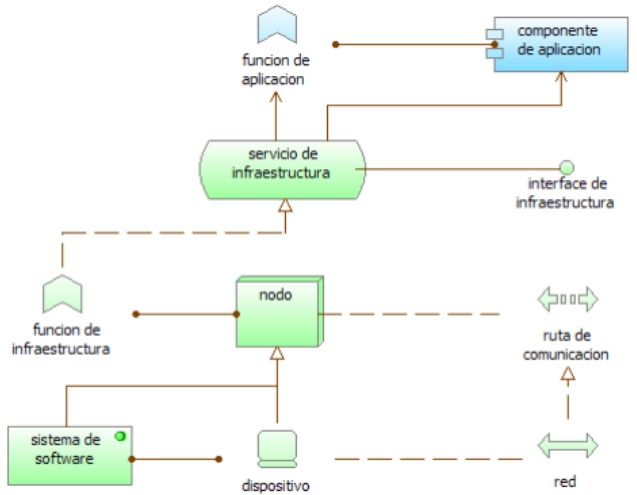
\includegraphics[width=0.5\linewidth]{imgs/puntos_vista/tecnologia/MMDUDI.jpg}}
	\caption{Metamodelo de uso de infraestructura}
\end{figure}

\subsubsection{Modelo de uso de infraestructura}

En este punto de vista se identifican los servicios de infraestructura principales que corresponden al servicio de notificaciones, generar reportes, establecer tiempos de acceso a la
aplicación, y gestionar los usuarios. Cada uno de los servicios de infraestructura entrega configuración y la funcionalidad requerida hacia los componentes de aplicación.


\begin{figure}[h]
	\centering
	\fcolorbox{black}{white}{
		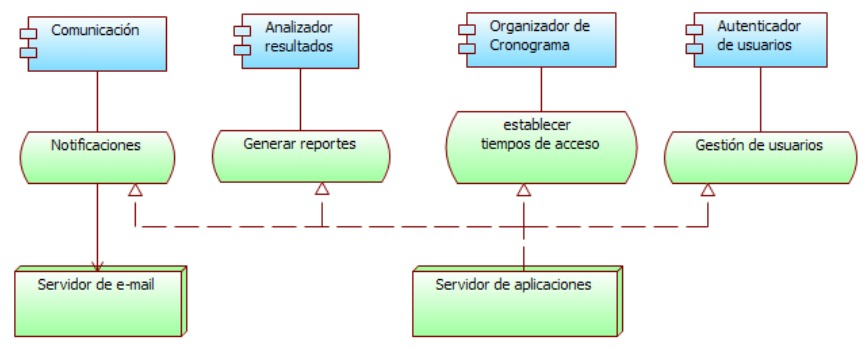
\includegraphics[width=0.5\linewidth]{imgs/puntos_vista/tecnologia/MDUDI.jpg}}
	\caption{Modelo de uso de infraestructura}
\end{figure}



\subsubsection{ Punto de vista de Implementación y despliegue}
El punto de vista de implementación y despliegue muestra como uno o más aplicaciones son realizadas sobre la infraestructura. Esto implica el mapeo de aplicaciones (lógicas) y componentes en artefactos (físicos). Esta vista juega un papel importante en el análisis del rendimiento y la escalabilidad debido a la relación entre la infraestructura y el mundo lógico de las aplicaciones.


\begin{figure}[h]
	\centering
	\fcolorbox{black}{white}{
		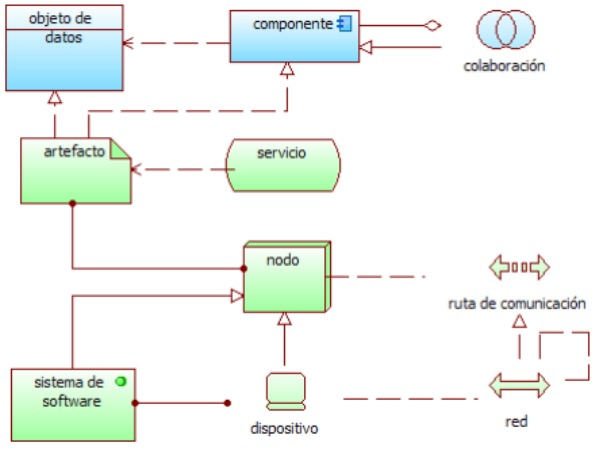
\includegraphics[width=0.5\linewidth]{imgs/puntos_vista/tecnologia/MMDIYD.jpg}}
	\caption{Metamodelo de implementación y despliegue}
\end{figure}

\subsubsection{Modelo de implementación y despliegue}

En este punto de vista, se muestra como todos los componentes son realizados por el nodo de servidor de aplicaciones, el componente de comunicación va a ser realizado por el nodo servidor de aplicaciones y tiene una relación de asociación con el nodo servidor de e-mail que
proveerá las configuraciones de software específico para el envío de notificaciones, resultados e información sobre el proceso.

\begin{figure}[h]
	\centering
	\fcolorbox{black}{white}{
		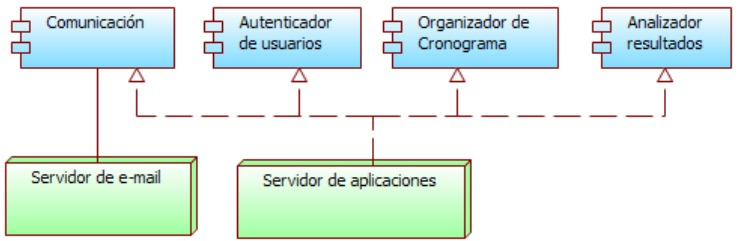
\includegraphics[width=0.5\linewidth]{imgs/puntos_vista/tecnologia/MDIYD.jpg}}
	\caption{Modelo de implementación y despliegue}
\end{figure}



\begin{table}[h]
	\begin{center}
		\begin{tabular}{ | m{7em} | m{8cm}|  } 
			\hline
			Interesados & Arquitectos de infraestructura, gerentes operativos 
			\\
			\hline
			Preocupaciones & Estabilidad, seguridad, dependencias, costos de la infraestructura
			\\
			\hline
			Propósito & Diseñar
			\\
			\hline
			Alcance & Una capa / aspecto múltiple
			\\
			\hline
		\end{tabular}
		\caption{Punto de Vista Tecnología}
		\label{tab:concepts}
	\end{center}
\end{table}

\textbf{Elementos que participan: }
\begin{itemize}
	\item Ubicación
	\item Nodo
	\item Colaboración tecnológica
	\item Dispositivo
	\item Software del sistema
	\item Interfaz tecnológica
	\item Red de comunicacion
	\item Camino
	\item Proceso tecnológico / función / interacción
	\item Servicio de tecnología
	\item Evento tecnológico
	\item Artefacto
\end{itemize}